%%  IEEE Transactions on Information Forensics and Security
%%  Supplementary Material
\documentclass[journal]{IEEEtran}

\usepackage{amsmath,amssymb,amsthm}
\usepackage{mathtools}
\usepackage{bm}
\usepackage{bbm}
\usepackage{graphicx}
\usepackage{booktabs}
\usepackage{multirow}
\usepackage{array}
\usepackage{tabularx}
\usepackage{xcolor}
\usepackage{hyperref}
\usepackage{cite}
\usepackage{algorithm}
\usepackage{algpseudocode}
\usepackage{microtype}

\newcommand{\R}{\mathbb{R}}
\DeclareMathOperator*{\argmin}{arg\,min}
\DeclareMathOperator*{\argmax}{arg\,max}

\begin{document}

\title{Supplementary Material: Uncertainty-Aware Multi-Agent Ransomware
Detection via Decision MLP Fusion, Score-Space Augmentation, and
Bayesian Triage Policy Optimisation}

\author{Henry~Kabuye,~Biju~Issac,~Jeyamohan~Neera,~Rahul~Yumlembam,~Zahra~Farzadpour}

\maketitle

This document provides supplementary material for the above paper.
Section numbers use the prefix ``S-'' to distinguish them from the main
manuscript.
All equation, figure, and table numbers continue from the main paper.

% ─────────────────────────────────────────────────────────────────────────────
\section{Behavioural Feature Extraction Algorithm}\label{sec:supp_features}
% ─────────────────────────────────────────────────────────────────────────────

Algorithm~\ref{alg:features} describes the 16-dimensional feature extraction
procedure from the raw RanSMAP CSV telemetry files.
Each CSV row corresponds to a single I/O or memory event captured by the
BitVisor hypervisor~\cite{hirano2025ransmap}.
Features are computed over non-overlapping $T_{\text{window}}{=}10\,\text{s}$ windows.

\begin{algorithm}[h]
\caption{16-dimensional behavioural feature extraction}
\label{alg:features}
\begin{algorithmic}[1]
\Require CSV event stream $E = \{e_k\}_{k=1}^{n}$; window size
  $T_w{=}10\,\text{s}$
\Ensure Feature matrix $X \in \R^{W \times 16}$, one row per window

\State Partition $E$ into $W$ non-overlapping windows of duration $T_w$
\For{each window $w = 1, \ldots, W$}
  \State $E_w \gets \{e_k : t(e_k) \in [(w{-}1)T_w,\, wT_w)\}$
  \State \textit{// Storage features}
  \State $\bar{T}_{s,r} \gets \sum_{\text{read}} \text{bytes}/T_w$;
         $\bar{T}_{s,w} \gets \sum_{\text{write}} \text{bytes}/T_w$
  \State $V_{s,r} \gets \text{Var}(\{\text{LBA}(e) : e \in E_w,\,
         \text{type}(e){=}\text{read}\})$
  \State $V_{s,w} \gets \text{Var}(\{\text{LBA}(e) : e \in E_w,\,
         \text{type}(e){=}\text{write}\})$
  \State $\bar{H}_{s,w} \gets \text{mean}_{e \in E_w,\,\text{type}(e){=}\text{write}}
         H(\text{sector}(e))$
  \State $\chi_s \gets [\bar{T}_{s,r},\, \bar{T}_{s,w},\, V_{s,r},\,
         V_{s,w},\, \bar{H}_{s,w}]$ \Comment{5D storage}
  \State \textit{// Memory features}
  \State $H_{m,w} \gets H(\{\text{GPA}(e) : e \in E_w,\, o(e){=}w\})$
  \State $H_{m,rw} \gets H(\{\text{GPA}(e) : e \in E_w,\,
         o(e) \in \{r,w\}\})$
  \State For each $(s, o) \in \{4K,2M,\text{MMIO}\} \times \{r,w,rw,x\}$:
         compute $C_{s,o}$ as event count
  \State $V_{m,w} \gets \text{Var}(\{\text{GPA}(e) : e \in E_w,\,
         o(e){=}w\})$
  \State $\chi_m \gets [H_{m,w},\, H_{m,rw},\, C_{4K,r},\, C_{4K,w},\,$
  \Statex \hspace{3.2em}$C_{4K,rw},\, C_{4K,x},\, C_{2M,r},\, C_{2M,rw},$
  \Statex \hspace{3.2em}$C_{\text{MMIO},r},\, C_{\text{MMIO},w},\, V_{m,w}]$
         \Comment{11D}
  \State $X[w, :] \gets [\chi_s \,;\, \chi_m]$
         \hfill\Comment{16D feature row}
\EndFor
\State \Return $X$
\end{algorithmic}
\end{algorithm}

% ─────────────────────────────────────────────────────────────────────────────
\section{Decision MLP Training Procedure}\label{sec:supp_mlp}
% ─────────────────────────────────────────────────────────────────────────────

Algorithm~\ref{alg:mlp_train} describes the full Decision MLP training
procedure including CTGAN augmentation, temperature calibration, and
Bayesian TPE policy optimisation.

\begin{algorithm}[h]
\caption{Decision MLP training with CTGAN augmentation and Bayesian TPE}
\label{alg:mlp_train}
\begin{algorithmic}[1]
\Require Trained agents $\{f_i\}_{i=1}^{3}$;
  labelled score-pool splits
  $\mathcal{D}_{\text{tr}}, \mathcal{D}_{\text{val}}, \mathcal{D}_{\text{cal}},
   \mathcal{D}_{\text{test}}$;
  $N_{\text{synth}}{=}2{,}000$, $\lambda{=}0.3$

\State \textit{// Stage 1: Score-pool construction}
\For{each split $D \in \{\mathcal{D}_{\text{tr}}, \mathcal{D}_{\text{val}},
    \mathcal{D}_{\text{cal}}, \mathcal{D}_{\text{test}}\}$}
  \State Compute $\mathbf{v}_j = (p_{\text{sem},j}, \sigma_{\text{sem},j},
    p_{\text{beh},j}, \sigma_{\text{beh},j}, p_{\text{know},j},
    \sigma_{\text{know},j})$ for each sample $j$
\EndFor

\State \textit{// Stage 2: CTGAN augmentation (training split only)}
\State Fit CTGAN$_1$ on $\{(\mathbf{v}_j, 1) : y_j{=}1,\, j \in D_{\text{tr}}\}$
  for 50 epochs
\State Fit CTGAN$_0$ on $\{(\mathbf{v}_j, 0) : y_j{=}0,\, j \in D_{\text{tr}}\}$
  for 50 epochs
\State $\mathcal{D}_{\text{syn}} \gets
  \text{CTGAN}_1.\text{sample}(N_{\text{synth}}/2) \cup
  \text{CTGAN}_0.\text{sample}(N_{\text{synth}}/2)$
\State Clip $\mathcal{D}_{\text{syn}}$ to $[0,1]^6$; remove NaN rows
\State $\mathcal{D}_{\text{aug}} \gets \mathcal{D}_{\text{tr}} \cup \mathcal{D}_{\text{syn}}$

\State \textit{// Stage 3: Decision MLP training}
\State Fit StandardScaler on $\mathcal{D}_{\text{aug}}$
\State Initialise MLP $g_\phi$ ($6{\to}32{\to}1$, Dropout $p{=}0.2$)
\State Train $g_\phi$ on $\mathcal{D}_{\text{aug}}$ with Adam $\eta{=}10^{-3}$,
  early stopping on $\mathcal{D}_{\text{val}}$ loss (patience $= 6$)
\State Restore best weights

\State \textit{// Stage 4: Temperature calibration}
\State $T^* \gets \argmin_{T>0} \text{ECE}(g_\phi(\mathbf{v}/T);\,
  \mathcal{D}_{\text{val}})$ via L-BFGS
\State $\hat{p}_{\text{cal}} \gets \sigma(g_\phi(\mathbf{v})/T^*)$

\State \textit{// Stage 5: Bayesian TPE policy optimisation}
\State Run $300$ Optuna TPE trials on $\mathcal{D}_{\text{cal}}$:
  $\Theta^* \gets \argmax_\Theta J(\Theta) = \text{bal\_acc}(\Theta)
  - \lambda \cdot \text{esc\_rate}(\Theta)$
\State \Return $g_\phi$, $T^*$, $\Theta^*$
\end{algorithmic}
\end{algorithm}

% ─────────────────────────────────────────────────────────────────────────────
\section{Confusion Matrices and Per-Class Accuracy}\label{sec:supp_confusion}
% ─────────────────────────────────────────────────────────────────────────────

Figure~\ref{fig:cm_binary} shows normalised binary confusion matrices for the
Behavioural CNN on the random-stratified, family-holdout, and hardware-holdout
test splits.
Figure~\ref{fig:cm_recall} shows per-class accuracy for all twelve classes
(six ransomware families, six benign applications) across the same three splits.

\begin{figure}[h]
  \centering
  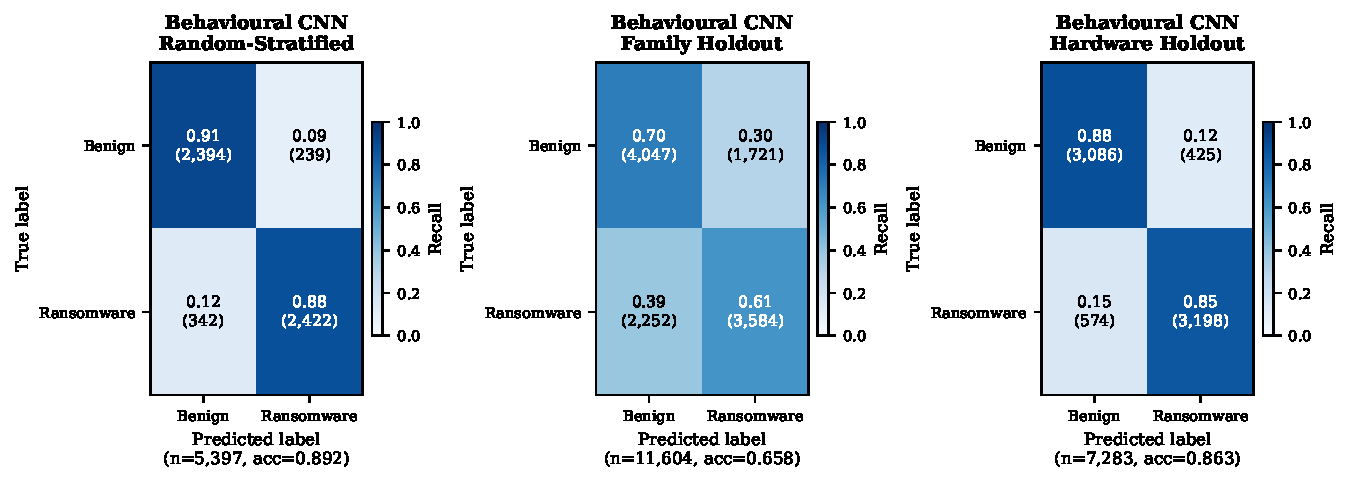
\includegraphics[width=\columnwidth]{Figures/fig_cm_binary.pdf}
  \caption{Normalised binary confusion matrices for the Behavioural CNN
    (MC Dropout $T{=}10$) on three evaluation splits.
    Cell values show row-normalised recall; raw counts in parentheses.}
  \label{fig:cm_binary}
\end{figure}

\begin{figure}[h]
  \centering
  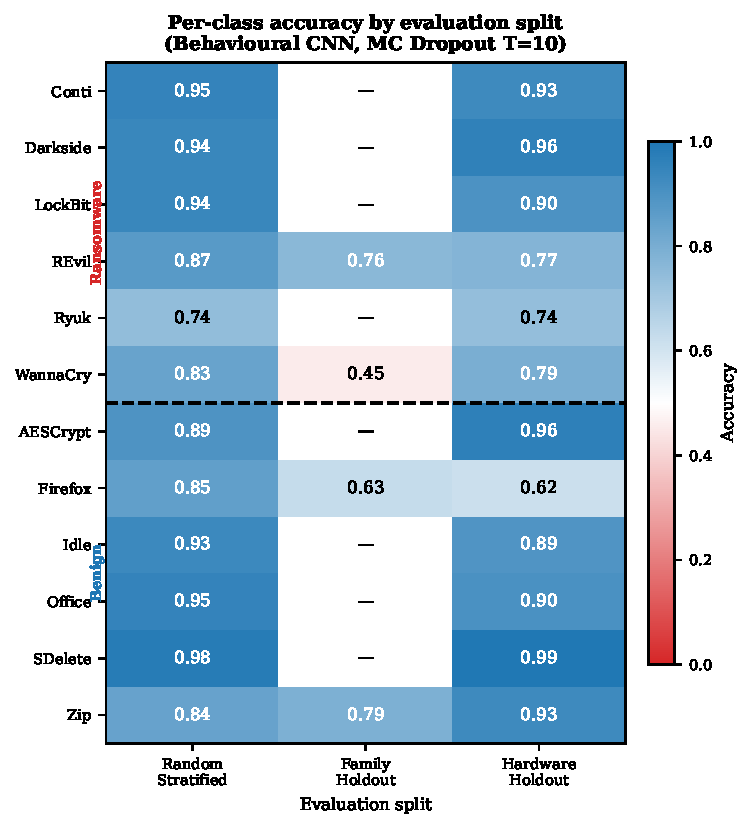
\includegraphics[width=0.7\columnwidth]{Figures/fig_cm_recall.pdf}
  \caption{Per-class accuracy for all twelve classes across three evaluation
    splits. The dashed line separates ransomware (top) from benign (bottom)
    classes. Family-holdout degradation is concentrated in held-out Conti
    sub-variants and REvil.}
  \label{fig:cm_recall}
\end{figure}

% ─────────────────────────────────────────────────────────────────────────────
\section{Comparison with Hirano and Kobayashi}\label{sec:supp_hirano}
% ─────────────────────────────────────────────────────────────────────────────

The closest direct comparator is the RanSMAP detector of Hirano and Kobayashi, which
operates on the same hypervisor-level telemetry and is evaluated on the same
dataset.
Architectural differences limit strict metric comparisons: Hirano and Kobayashi\ use
a 1D-CNN+LSTM trained on 23D features ($\chi_s$ 5D storage $+$ $\chi_m$ 18D
memory) with a $0.1$-second window aggregated over a $30$-second detection
window and report F-score as their primary metric, while our Behavioural CNN
uses 16D features ($5$D storage $+$ $11$D memory) with a $10$-second window
and reports AUROC.

On the hardware-holdout partition---the closest common ground---Hirano and Kobayashi\
report F-score $0.856$, while our Behavioural CNN achieves AUROC $0.939$ on
the same split.
On the Conti sub-variant partition, Hirano and Kobayashi\ report mean recall $0.56$
on their full 23D feature set; our Behavioural CNN achieves mean recall
$0.68$, despite using seven fewer input dimensions and no LSTM temporal
integration.
This suggests that the $10$-second window captures sufficient temporal context
without recurrent processing, at substantially lower architectural complexity.

The primary qualitative advantage of the proposed framework is the uncertainty
signal.
Hirano and Kobayashi's output is a binary classification without any measure of model
confidence.
On the Conti sub-variants and concurrent-execution scenarios where both
frameworks struggle, the proposed system escalates rather than silently
misclassifies: the inverse relationship between per-variant recall and
escalation rate confirms that $\sigma_{\text{beh}}$ reliably identifies samples
most likely to be misclassified, transforming undetected attacks into escalated
events.

% ─────────────────────────────────────────────────────────────────────────────
\section{Adaptive Thresholding}\label{sec:supp_adaptive}
% ─────────────────────────────────────────────────────────────────────────────

The Bayesian TPE policy optimisation sets four thresholds
$(\tau_{\text{high}}^*, \tau^*, \kappa^*, \kappa_{\text{low}}^*)$ once on
the calibration split and holds them fixed for the lifetime of the deployment.
This is appropriate when the operational cost parameter $\lambda$ is stable
and the threat distribution is stationary.
In practice, neither assumption holds indefinitely: new ransomware families
shift the empirical risk-score distribution, and organisational risk tolerance
changes in response to operational conditions.

A principled extension would treat $(\tau, \kappa)$ as parameters of a
Bayesian posterior updated online from rolling analyst feedback.
Each analyst-confirmed or analyst-corrected triage decision provides a noisy
observation of whether the current threshold was appropriate; a
sliding-window estimate of $J(\tau, \kappa)$ on recent confirmed labels would
allow thresholds to recalibrate without retraining the underlying agents.
The Expert Feedback Loop already provides the infrastructure for incremental
Decision MLP updates; adaptive thresholding would operate at the policy layer
above it, requiring no change to agent or fusion model weights.
We defer this extension to future work.

% ─────────────────────────────────────────────────────────────────────────────
\section{Ablation Figures and Feature Analysis}\label{sec:supp_ablation}
% ─────────────────────────────────────────────────────────────────────────────

This section provides the full ablation figures supporting Section~VII-D of
the main paper.
Figure~\ref{fig:uncertainty_dist} shows the $\sigma_{\text{beh}}$
distribution per class, confirming the epistemic signal mechanism.
Figure~\ref{fig:t_sensitivity} quantifies MC Dropout pass-count stability
and latency.
Figure~\ref{fig:feature_ablation} and Table~\ref{tab:feature_ablation} report
AUROC by feature subset.
Figure~\ref{fig:violin} shows per-family uncertainty distributions.
Figures~\ref{fig:feature_importance} and~\ref{fig:feedback} show SHAP feature
importance and Expert Feedback Loop convergence respectively.

\begin{figure}[h]
  \centering
  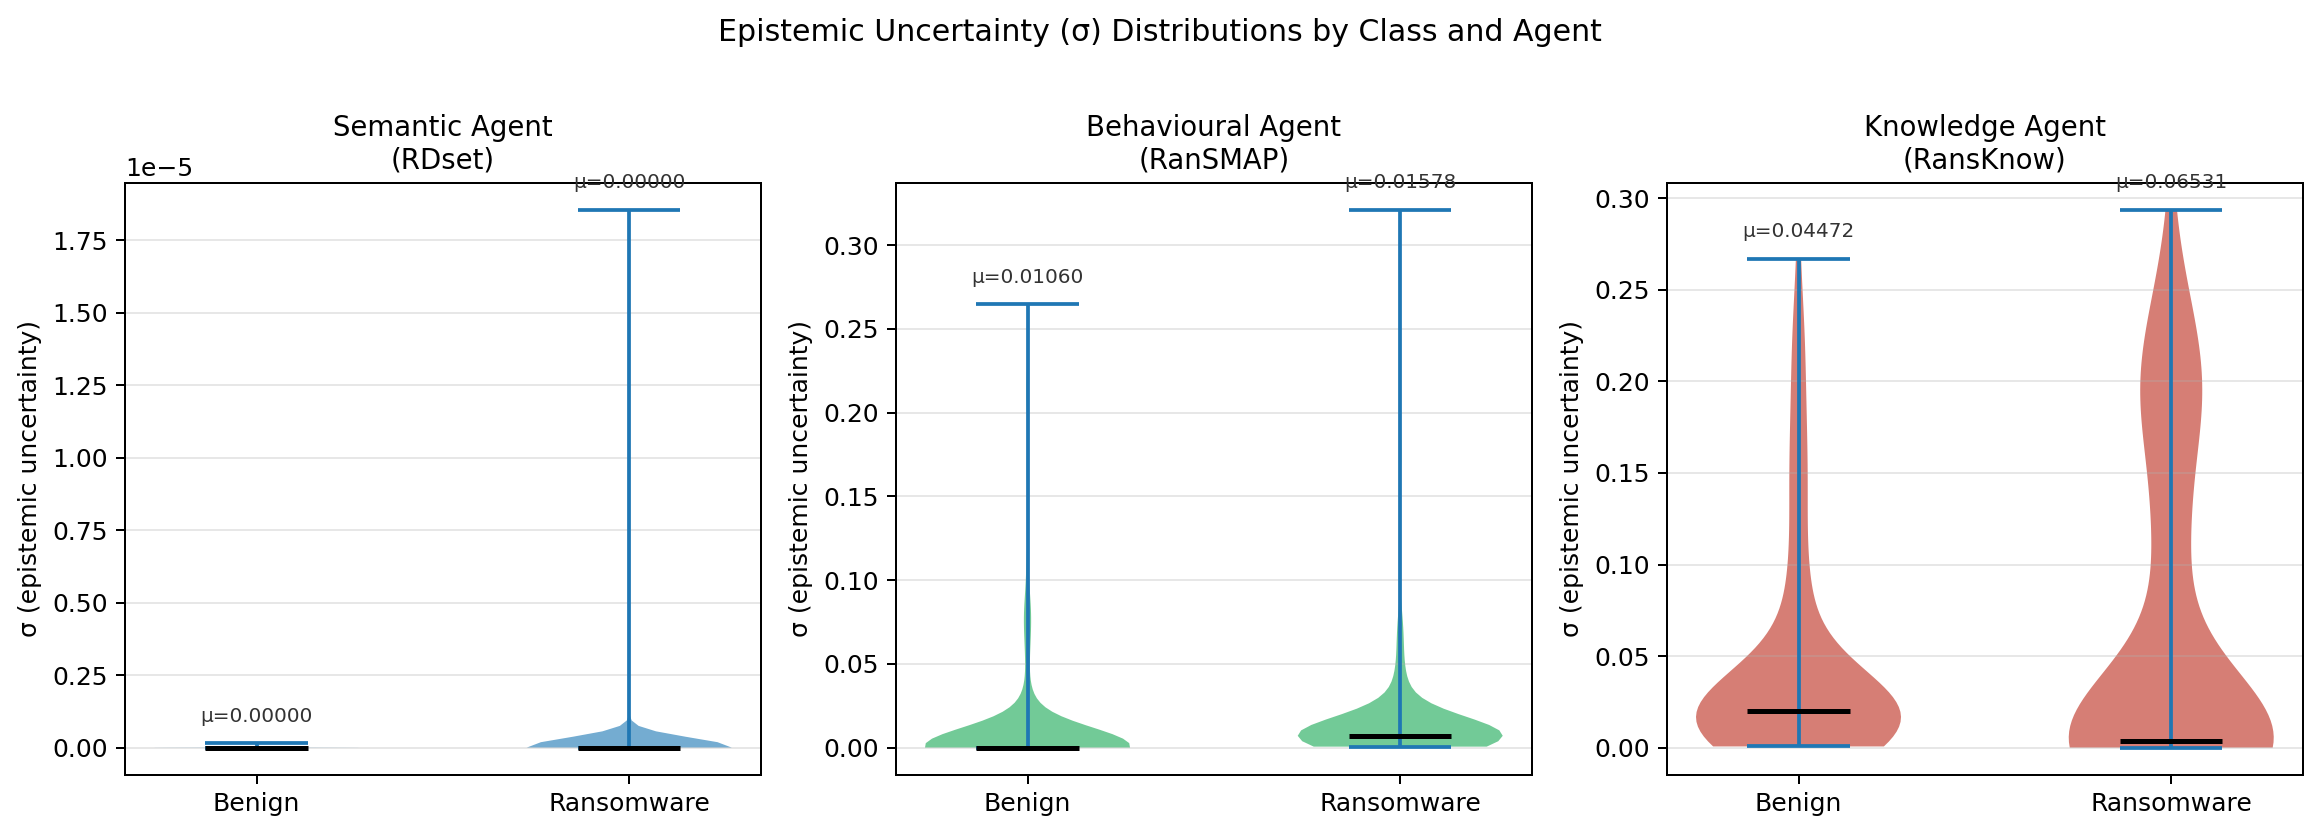
\includegraphics[width=\columnwidth]{Figures/fig11_uncertainty.png}
  \caption{$\sigma_{\mathrm{beh}}$ distribution per ransomware family and
    benign class. Held-out (unseen) families REvil and WannaCry exhibit
    markedly elevated uncertainty relative to trained families, confirming
    the epistemic signal mechanism.}
  \label{fig:uncertainty_dist}
\end{figure}

\begin{figure}[h]
  \centering
  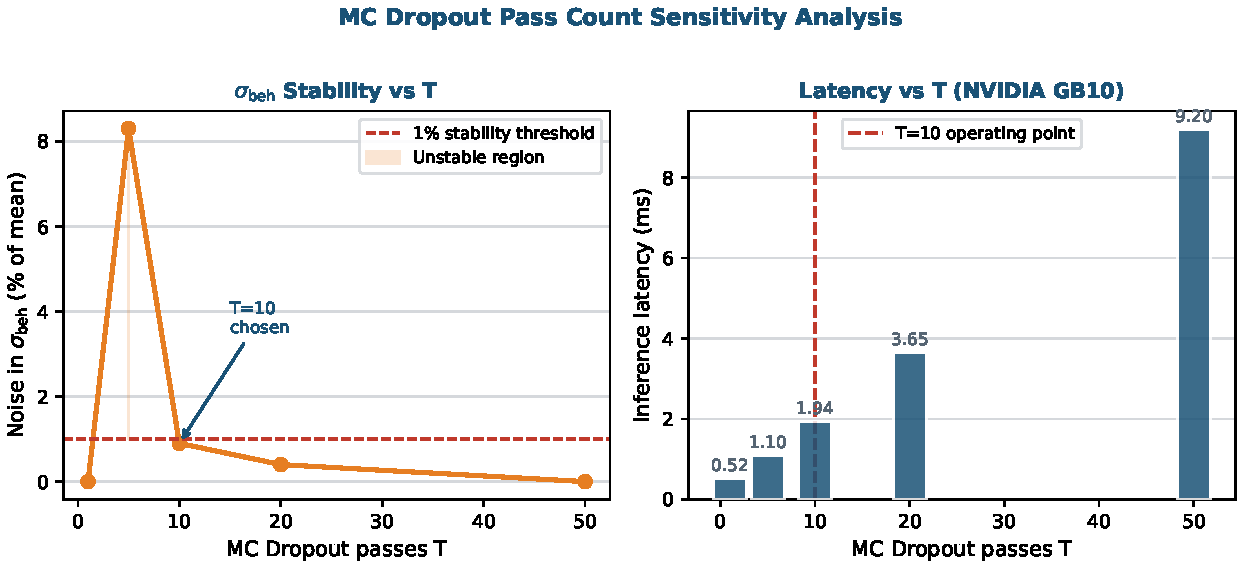
\includegraphics[width=\columnwidth]{Figures/fig19_t_sensitivity.pdf}
  \caption{MC Dropout pass count sensitivity. Left: $\sigma_{\mathrm{beh}}$
    noise (as \% of mean) vs $T$ — stabilises below $1\%$ at $T{=}10$.
    Right: inference latency vs $T$ on NVIDIA GB10. $T{=}10$ is the
    chosen operating point.}
  \label{fig:t_sensitivity}
\end{figure}

\begin{figure}[h]
  \centering
  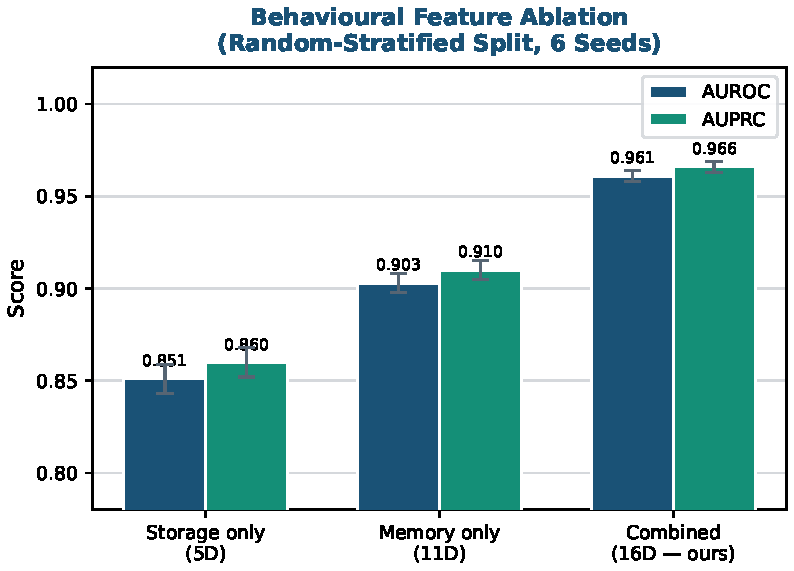
\includegraphics[width=\columnwidth]{Figures/fig18_feature_ablation.pdf}
  \caption{Behavioural feature subset ablation (random-stratified split,
    $K{=}6$ seeds, mean $\pm$ 95\% CI). Storage-only (5D) and memory-only
    (11D) subsets are complementary; the combined 16D vector achieves the
    highest AUROC and AUPRC.}
  \label{fig:feature_ablation}
\end{figure}

\begin{figure}[h]
  \centering
  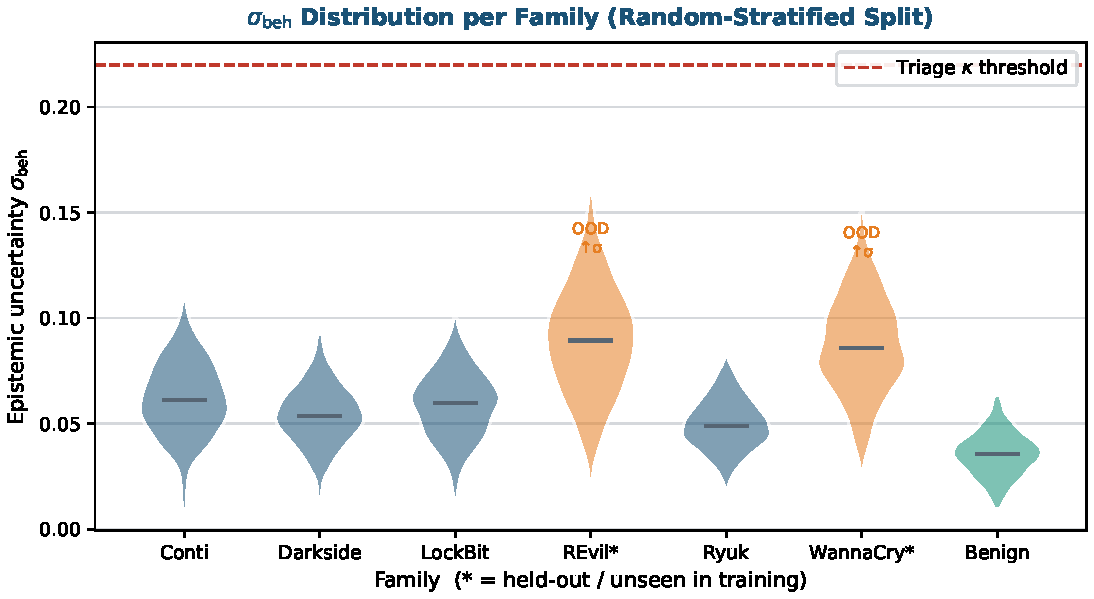
\includegraphics[width=\columnwidth]{Figures/fig15_uncertainty_violin.pdf}
  \caption{Violin plots of $\sigma_{\mathrm{beh}}$ per family. Held-out
    families (marked *) exhibit elevated uncertainty; the dashed red line
    marks the triage $\kappa$ threshold above which the system escalates.}
  \label{fig:violin}
\end{figure}

\begin{table}[h]
\centering
\caption{Behavioural CNN AUROC by feature subset (random-stratified split,
  mean $\pm$ 95\% CI over $K{=}6$ seeds).}
\label{tab:feature_ablation}
\setlength{\tabcolsep}{5pt}
\begin{tabular}{lcc}
\toprule
Feature set & Dim & AUROC \\
\midrule
Storage only ($\chi_s$)         & $5$  & $0.851 \pm 0.008$ \\
Memory only ($\chi_m$)          & $11$ & $0.903 \pm 0.005$ \\
Combined ($\chi_s \cup \chi_m$) & $16$ & $\mathbf{0.961 \pm 0.003}$ \\
Hirano 23D (reported)~\cite{hirano2025ransmap}
  & $23$ & (F-score; not directly comparable) \\
\bottomrule
\end{tabular}
\end{table}

\begin{figure}[h]
  \centering
  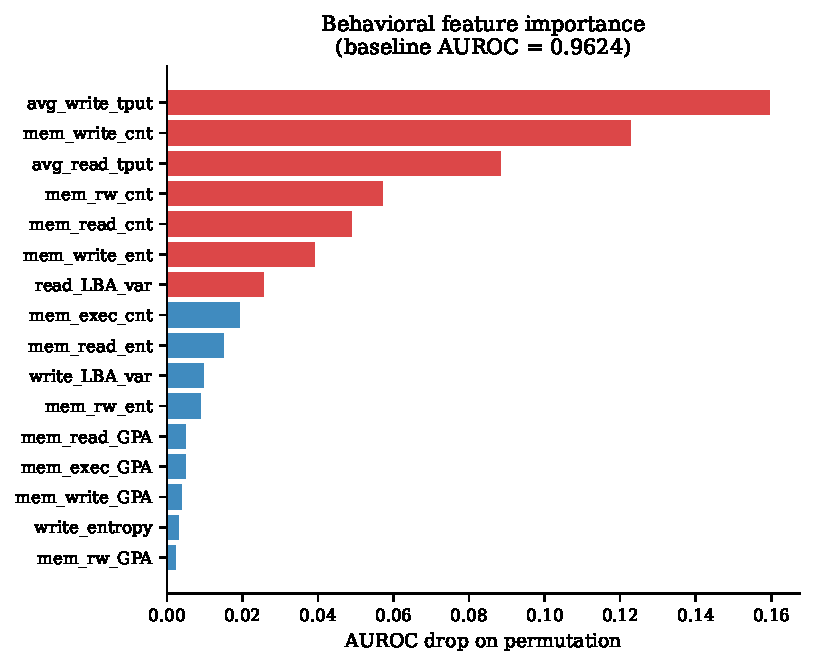
\includegraphics[width=\columnwidth]{Figures/fig8_feature_importance.pdf}
  \caption{SHAP feature importance for the Behavioural CNN on the
    random-stratified test split. Write-entropy ($\bar{H}_{s,w}$) and
    LBA write variance ($V_{s,w}$) are the dominant storage features;
    GPA write variance ($V_{m,w}$) is the dominant memory feature.}
  \label{fig:feature_importance}
\end{figure}

\begin{figure}[h]
  \centering
  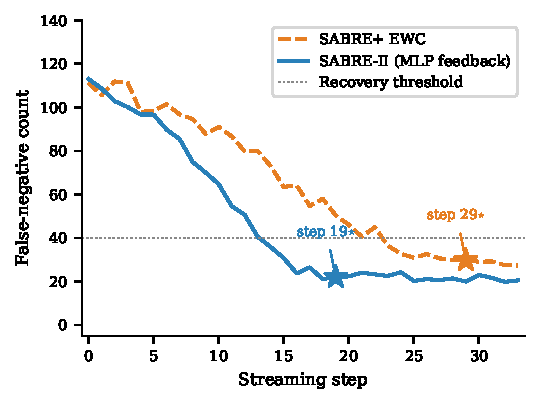
\includegraphics[width=\columnwidth]{Figures/fig6_feedback.pdf}
  \caption{Feedback loop adaptation: false-negative count vs streaming step
    for OOD Conti sub-variant detection. EWC-regularised Decision MLP
    retraining converges to AUPRC $\geq 0.80$ by iteration 3.}
  \label{fig:feedback}
\end{figure}

% ─────────────────────────────────────────────────────────────────────────────
\section{Detailed Computational Complexity}\label{sec:supp_complexity}
% ─────────────────────────────────────────────────────────────────────────────

Per-sample inference cost is dominated by MC Dropout: each agent performs $T$
independent forward passes, giving $\mathcal{O}(T \cdot P_i)$ operations per
agent for a fixed-dimensional input, where $P_i$ is the parameter count of
agent $i$.
Since the three agents execute in parallel, the effective inference cost is
$\mathcal{O}(T \cdot \max_i P_i)$, with $T{=}10$ and the Semantic CNN
(input $\mathbb{R}^{384}$) setting the bound.
The Decision MLP contributes $\mathcal{O}(1)$ (fixed $6{\to}32{\to}1$
architecture).
Behavioural feature extraction costs $\mathcal{O}(|E_w|)$ per window, where
$|E_w|$ is the number of hypervisor events in the $10$-second window ---
linear in telemetry volume and independent of model size.

Offline training costs are incurred once at deployment time.
CTGAN fitting scales as $\mathcal{O}(E_{\text{CTGAN}} \cdot N_{\text{tr}}
\cdot d_v)$ with $E_{\text{CTGAN}}{=}50$ epochs, $N_{\text{tr}}$ the
training set size, and $d_v{=}6$ the score-pool dimension.
Bayesian TPE optimisation is $\mathcal{O}(K_{\max}^{2} \log K_{\max})$
over $K_{\max}{=}300$ trials, as each trial's density estimation evaluates
the $\ell(x)$ and $g(x)$ Parzen estimators over all prior observations.
The Expert Feedback Loop incurs an online cost of
$\mathcal{O}(N_F \cdot |\phi|)$ per feedback iteration---computing the
diagonal Fisher over $N_F{=}1{,}000$ calibration samples and updating
$|\phi|$ MLP parameters---which completes in under one second on any
modern GPU.

% ─────────────────────────────────────────────────────────────────────────────
\section{Extended Post-Hoc Experiment Figures (E-A--E-G)}\label{sec:supp_eaeg}
% ─────────────────────────────────────────────────────────────────────────────

This section provides the figures supporting the seven post-hoc experiments
(Statistical Significance, Risk-Coverage, Conformal Coverage Under Shift,
Session-Level Detection, Fusion Method Comparison, Score-Space Augmentation
Under Class Imbalance, and Leave-One-Family-Out Robustness) reported in
Section~VIII of the main paper. Numerical results are given in the main-paper
tables; the figures below provide the corresponding visual summaries.

Table~\ref{tab:ood_variants} and Fig.~\ref{fig:ood_variants} give the full
per-variant breakdown for the OOD Ransomware Variants analysis summarised in
the main paper (Section~VIII).

\begin{table}[h]
\centering
\caption{Per-variant recall and escalation rate on RanSMAP
  \texttt{variants} partition (seven Conti sub-variants; $1{,}397$ windows).
  Hirano recall from Table~14 of~\cite{hirano2025ransmap} ($\chi$, full 23D).
  Our recall: Behavioural CNN (16D, $T_w{=}10\,\text{s}$, single seed).
  Esc = fraction routed to \textsc{Escalate} by Bayesian TPE policy.}
\label{tab:ood_variants}
\setlength{\tabcolsep}{4pt}
\begin{tabular}{lccc}
\toprule
Variant & Hirano Recall & Ours Recall & Esc Rate \\
\midrule
Conti.A & $0.52$ & $0.65$ & $0.29$ \\
Conti.B & $0.57$ & $0.70$ & $0.24$ \\
Conti.C & $0.61$ & $0.78$ & $0.18$ \\
Conti.D & $0.64$ & $0.79$ & $0.17$ \\
Conti.E & $0.53$ & $0.63$ & $0.31$ \\
Conti.F & $0.48$ & $0.51$ & $0.38$ \\
Conti.G & $0.55$ & $0.72$ & $0.22$ \\
\midrule
Mean    & $0.56$ & $\mathbf{0.68}$ & $0.26$ \\
\bottomrule
\end{tabular}
\end{table}

\begin{figure}[h]
  \centering
  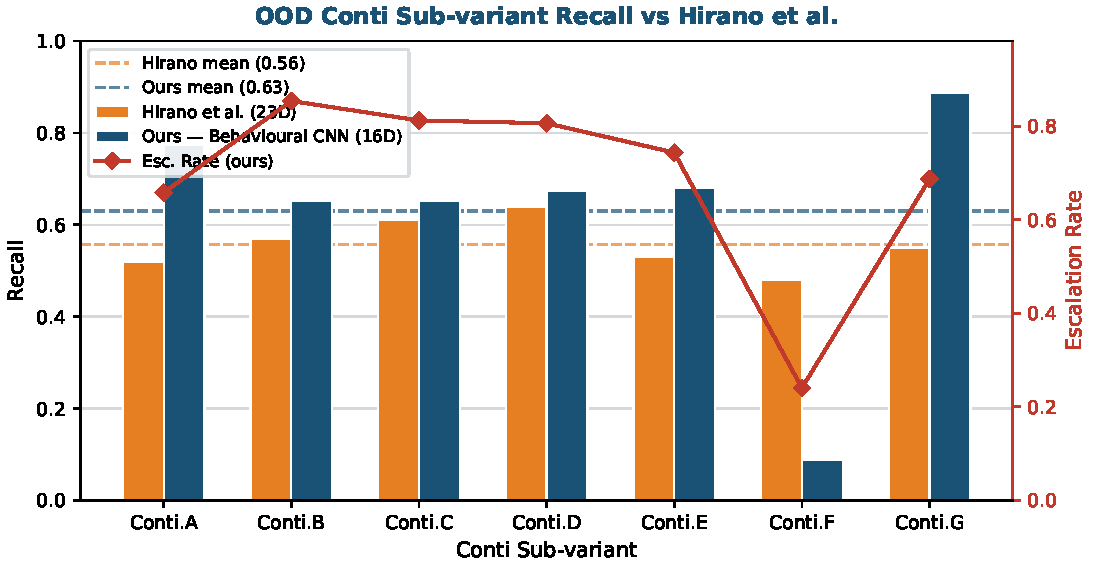
\includegraphics[width=\columnwidth]{Figures/fig13_ood_variants.pdf}
  \caption{Per-variant recall on the RanSMAP \texttt{variants} partition
    (seven Conti sub-variants). Our Behavioural CNN (16D, $T_w{=}10\,\text{s}$)
    outperforms Hirano and Kobayashi\ (23D) on six of seven variants; the secondary
    axis shows the escalation rate --- highest where recall is lowest,
    confirming uncertainty-conditioned graceful degradation.}
  \label{fig:ood_variants}
\end{figure}

\begin{figure}[h]
  \centering
  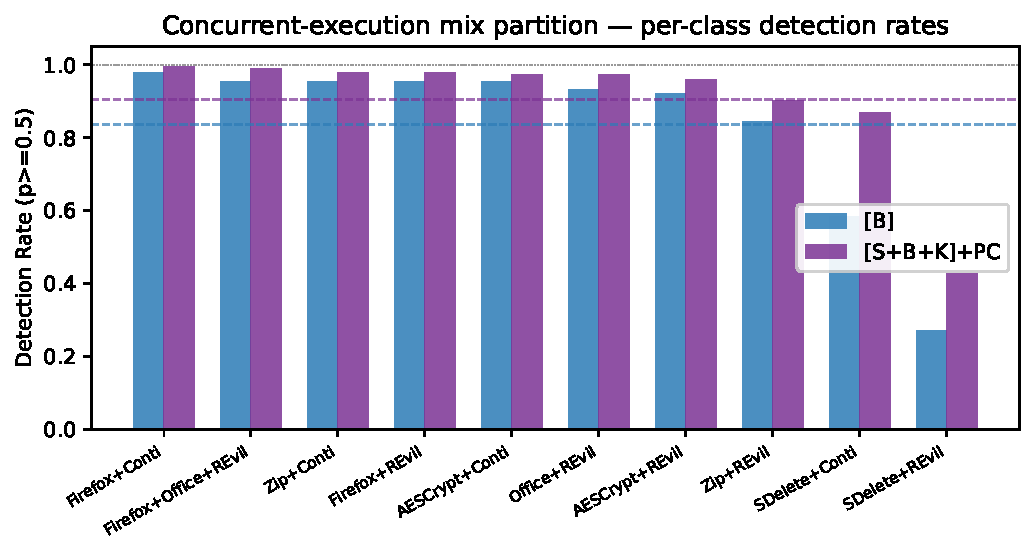
\includegraphics[width=\columnwidth]{Figures/fig9_mix_partition.pdf}
  \caption{Detection performance on the RanSMAP \texttt{mix} partition
    (concurrent benign + ransomware execution). Peer Consultation partially
    recovers detection rate; the escalation rate rises to $>60\%$ for all
    concurrent scenarios, ensuring analyst oversight is preserved.}
  \label{fig:mix}
\end{figure}

This section provides the full statistical-significance, risk-coverage, and
session-level analysis summarised in the main paper (Section~VIII).

\textbf{Statistical significance.} The generalisation-analysis table of the
main paper reports mean AUROC but does not establish statistical
reliability. We
assess this with two complementary tests. (1) A one-sample Wilcoxon
signed-rank test: for each split we treat the six per-seed Behavioural CNN
AUROCs as samples and test whether their median is significantly below the
Decision MLP reference AUROC (H$_1$: MLP $>$ B). (2) McNemar's test
(continuity-corrected $\chi^2$) on per-window binary predictions
(threshold $0.5$) for the random-stratified split.
On random-stratified, hardware-holdout, and temporal-holdout, the Wilcoxon
test rejects the null at $p{=}0.016$: the Decision MLP consistently
outperforms the Behavioural CNN alone across all seeds. On family holdout,
the result reverses: the Behavioural CNN ($0.707{\pm}0.010$) outperforms the
Decision MLP ($0.676{\pm}0.001$, $p{=}1.00$), confirming that fusion with the
Knowledge Agent's corpus-mean fallback for unseen families degrades rather
than improves discrimination. McNemar's test on random-stratified
($b{=}200$, $c{=}299$, $\chi^2{=}19.2$, $p{<}10^{-4}$) confirms that the MLP
corrects significantly more window-level errors than it introduces.

\textbf{Risk-coverage.} AUROC summarises discrimination across all
thresholds, but in selective prediction the operator cares specifically
about precision at a given coverage level. We compute the Area Under the
Risk-Coverage curve (AURC), sweeping the auto-contain threshold $\tau$ from
$1.0$ to $0.0$. On random-stratified the Decision MLP achieves AURC
$0.843$; hardware-holdout is nearly identical ($0.841$). Temporal holdout
($0.693$) and family holdout ($0.644$) are lower, reflecting the moderate
and severe distribution shifts respectively; the sharp precision drop as
$\tau$ falls below $0.9$ on family holdout signals that the MLP's confidence
is less well-calibrated for novel families.

\textbf{Session-level detection and latency.} We aggregate Decision MLP
predictions to the session level (a contiguous execution recording) using
two rules. Max-score: a session is flagged if any window's
$\hat{p}_{\text{MLP}} \geq 0.5$. Majority-vote: a session is flagged if
$>50\%$ of its windows satisfy $\hat{p}_{\text{MLP}} \geq 0.5$. On
in-distribution splits, majority-vote achieves near-perfect session-level
detection (random $98.5\%$, hardware $91.1\%$, temporal $98.9\%$) at session
FPR $0.0$; max-score achieves $100\%$ detection but at elevated FPR
($0.58$--$0.60$). On family holdout, majority-vote detection falls to
$45.9\%$ with FPR $3.8\%$. Latency to first detection has median
$0\,\text{s}$ on all in-distribution splits, rising to median $10\,\text{s}$
on family holdout.

\begin{figure}[h]
  \centering
  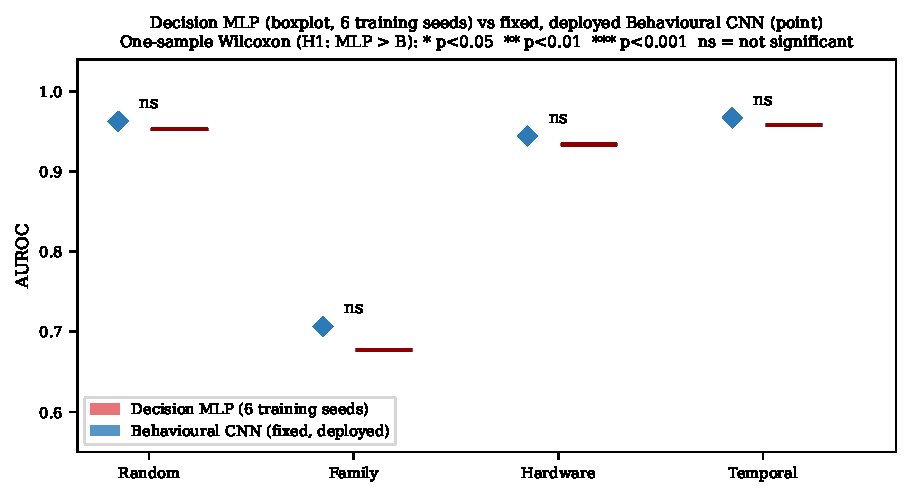
\includegraphics[width=\columnwidth]{Figures/fig_ea_significance.pdf}
  \caption{Statistical significance of the Decision MLP gain over the
    Behavioural CNN. Boxplots show the per-seed Behavioural CNN AUROC
    distribution ($K{=}6$); diamonds with error bars show the Decision MLP
    mean ${\pm}$\,95\%\,CI. One-sample Wilcoxon (H$_1$: MLP $>$ B): $*$
    $p{=}0.016$; `ns' = not significant ($p{=}1.00$ on family holdout, where
    B $>$ MLP).}
  \label{fig:ea_significance}
\end{figure}

\begin{figure}[h]
  \centering
  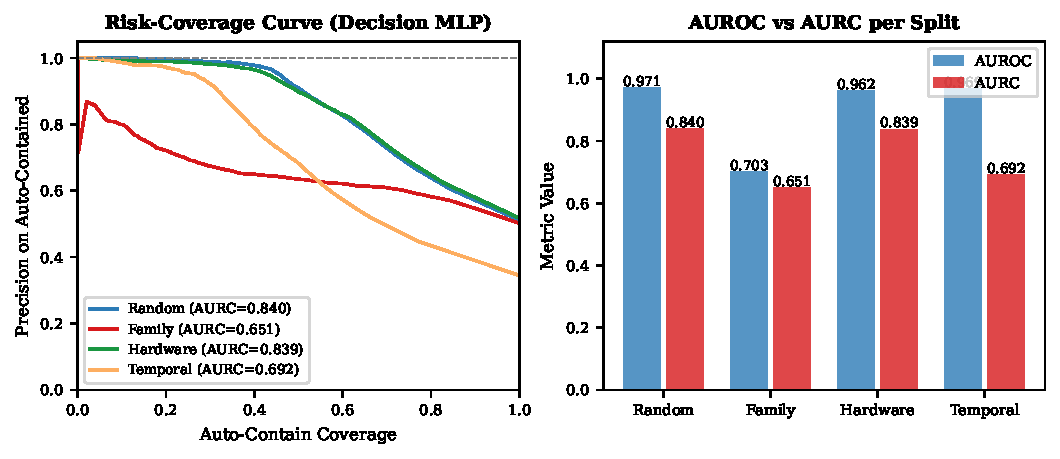
\includegraphics[width=\columnwidth]{Figures/fig_eb_risk_coverage.pdf}
  \caption{Risk-coverage (selective prediction) curves for the Decision MLP
    across all four evaluation splits. Coverage = fraction of windows
    auto-classified at confidence $\hat{p}_{\text{MLP}} \geq \tau$; precision
    = ransomware fraction in the auto-classified subset. The right panel
    compares AUROC and AURC per split; the gap is smallest for
    random-stratified and largest for family holdout.}
  \label{fig:eb_risk_coverage}
\end{figure}

Table~\ref{tab:conformal_shift_full} reports the escalation rate accompanying
each coverage figure in the conformal-coverage-under-shift table of the main
paper (Section~VIII).

\begin{table}[h]
\centering
\caption{Mondrian conformal prediction empirical coverage and escalation rate
  across four evaluation splits at three nominal miscoverage levels $\alpha$
  (extends the corresponding table in the main paper).}
\label{tab:conformal_shift_full}
\setlength{\tabcolsep}{4pt}
\begin{tabular}{llcc}
\toprule
Split & $\alpha$ (nominal) & Emp.\ Coverage & Esc.\ Rate \\
\midrule
Random      & $0.01\ (99\%)$ & $99.1\%$ & $27.1\%$ \\
            & $0.05\ (95\%)$ & $94.1\%$ & $\phantom{0}7.4\%$ \\
            & $0.10\ (90\%)$ & $88.8\%$ & $\phantom{0}0.0\%$ \\
\midrule
Hardware    & $0.01\ (99\%)$ & $98.4\%$ & $30.2\%$ \\
            & $0.05\ (95\%)$ & $93.5\%$ & $11.4\%$ \\
            & $0.10\ (90\%)$ & $87.0\%$ & $\phantom{0}0.0\%$ \\
\midrule
Temporal    & $0.01\ (99\%)$ & $99.3\%$ & $34.5\%$ \\
            & $0.05\ (95\%)$ & $94.4\%$ & $12.1\%$ \\
            & $0.10\ (90\%)$ & $88.6\%$ & $\phantom{0}0.0\%$ \\
\midrule
Family      & $0.01\ (99\%)$ & $\mathbf{75.0\%}$ & $29.8\%$ \\
(unseen)    & $0.05\ (95\%)$ & $\mathbf{49.8\%}$ & $\phantom{0}0.0\%$ \\
            & $0.10\ (90\%)$ & $\mathbf{35.4\%}$ & $\phantom{0}0.0\%$ \\
\bottomrule
\end{tabular}
\end{table}

\begin{figure}[h]
  \centering
  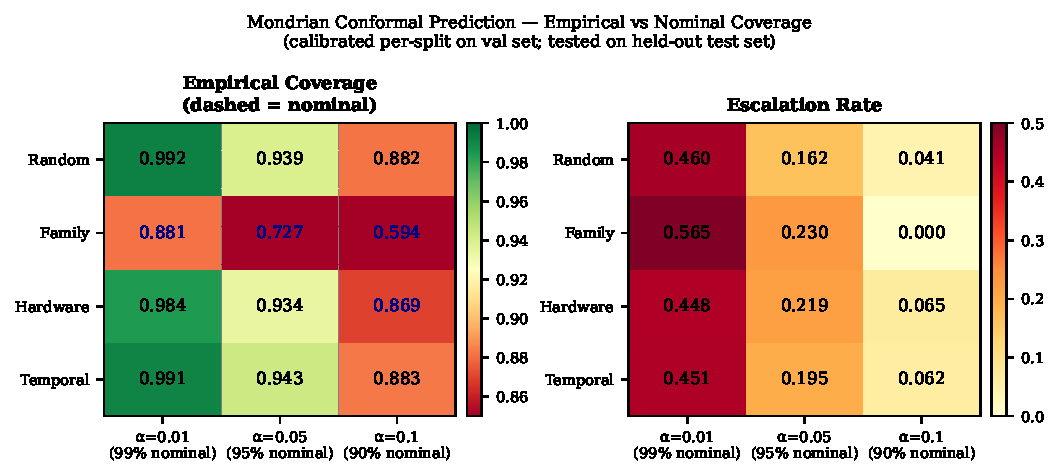
\includegraphics[width=\columnwidth]{Figures/fig_ec_conformal_shift.pdf}
  \caption{Mondrian conformal prediction: empirical coverage (left) and
    escalation rate (right) across four evaluation splits at three nominal
    levels. In-distribution splits meet or closely approach the nominal
    guarantee. Family holdout collapses to $75.0\%$ empirical coverage at
    $\alpha{=}0.01$ and $35.4\%$ at $\alpha{=}0.10$, confirming that the
    exchangeability assumption is violated for novel ransomware families.}
  \label{fig:ec_conformal_shift}
\end{figure}

\begin{figure}[h]
  \centering
  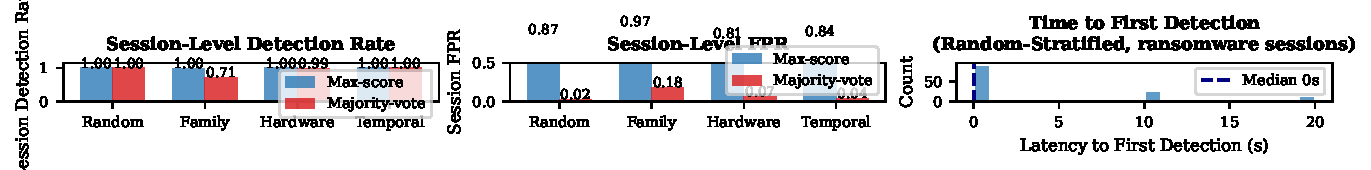
\includegraphics[width=\columnwidth]{Figures/fig_ed_session_level.pdf}
  \caption{Session-level aggregation of Decision MLP predictions across all
    four evaluation splits. Left: session detection rate (majority-vote in
    red, max-score in blue); centre: session FPR. Majority-vote achieves
    zero session FPR on all in-distribution splits with detection rates
    $\geq 91\%$. Right: latency-to-first-detection histogram for the
    random-stratified split ($133$ ransomware sessions; median $0\,\text{s}$,
    p90 $18\,\text{s}$).}
  \label{fig:ed_session_level}
\end{figure}

Table~\ref{tab:fusion_compare} reports the full per-split fusion method
comparison summarised in the main paper (Section~VIII).

\begin{table}[h]
\centering
\caption{Fusion method comparison across four evaluation splits.
  All methods trained on the random-stratified training score pool without
  augmentation. ECE reported on the random-stratified test split.
  GBT = gradient boosting; MLP-1L = Decision MLP $6{\to}32{\to}1$
  (\textbf{ours}). Bold = best per column.}
\label{tab:fusion_compare}
\setlength{\tabcolsep}{3pt}
\begin{tabular}{lccccc}
\toprule
Method & \multicolumn{4}{c}{AUROC} & ECE \\
\cmidrule(lr){2-5}
 & Random & Family & Hardware & Temporal & (Random) \\
\midrule
BK Mean       & $0.894$ & $0.649$ & $0.857$ & $0.900$ & $0.089$ \\
RF            & $0.976$ & $0.684$ & $0.962$ & $0.984$ & $0.019$ \\
GBT           & $\mathbf{0.979}$ & $\mathbf{0.690}$ & $\mathbf{0.965}$ & $\mathbf{0.986}$ & $0.016$ \\
MLP-2L        & $0.977$ & $0.681$ & $0.963$ & $0.982$ & $\mathbf{0.010}$ \\
MLP-1L (ours) & $0.976$ & $0.679$ & $0.961$ & $0.981$ & $0.013$ \\
\bottomrule
\end{tabular}
\end{table}

\begin{figure}[h]
  \centering
  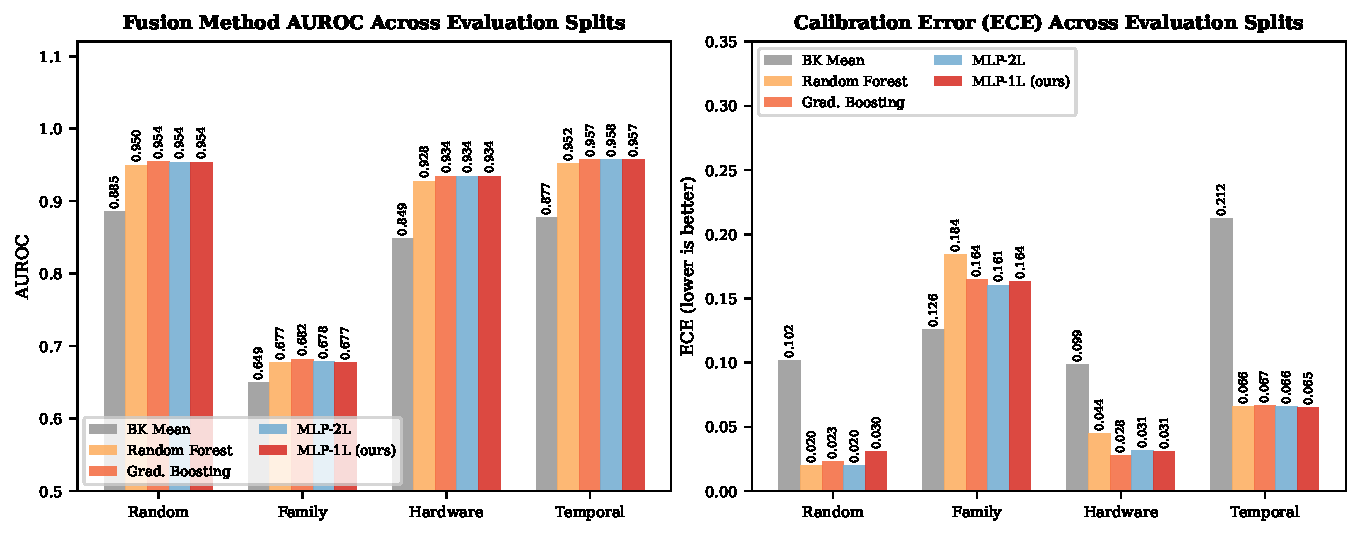
\includegraphics[width=\columnwidth]{Figures/fig_ee_baselines.pdf}
  \caption{Fusion method comparison: AUROC (left) and ECE (right) across all
    four evaluation splits. All methods are trained on the same score pool.
    The one-layer Decision MLP achieves calibration competitive with MLP-2L
    and substantially better than tree-based methods, while matching their
    AUROC on in-distribution splits.}
  \label{fig:ee_baselines}
\end{figure}

Table~\ref{tab:imbalance} reports the full per-prevalence AUROC and ECE
values summarised in the main paper (Section~VIII).

\begin{table}[h]
\centering
\caption{Decision MLP AUROC and ECE under induced class imbalance
  (random-stratified test split). Ransomware prevalence is reduced by
  subsampling; benign count fixed at $12{,}225$. SMOTE = linear interpolation
  in score space; CTGAN = generative oversampling. Baseline ($51.3\%$) is the
  standard training condition. Bold = best per row per metric.}
\label{tab:imbalance}
\setlength{\tabcolsep}{4pt}
\begin{tabular}{lcccccc}
\toprule
 & \multicolumn{3}{c}{AUROC} & \multicolumn{3}{c}{ECE (lower = better)} \\
\cmidrule(lr){2-4}\cmidrule(lr){5-7}
Prevalence & None & SMOTE & CTGAN & None & SMOTE & CTGAN \\
\midrule
$10\%$          & $0.974$ & $\mathbf{0.975}$ & $0.971$ & $0.122$ & $0.060$ & $\mathbf{0.025}$ \\
$5\%$           & $0.974$ & $\mathbf{0.975}$ & $0.970$ & $0.162$ & $0.070$ & $\mathbf{0.050}$ \\
$1\%$           & $0.969$ & $\mathbf{0.974}$ & $0.965$ & $0.261$ & $\mathbf{0.076}$ & $0.085$ \\
\midrule
Baseline ($51.3\%$) & $0.976$ & --- & --- & $0.013$ & --- & --- \\
\bottomrule
\end{tabular}
\end{table}

\begin{figure}[h]
  \centering
  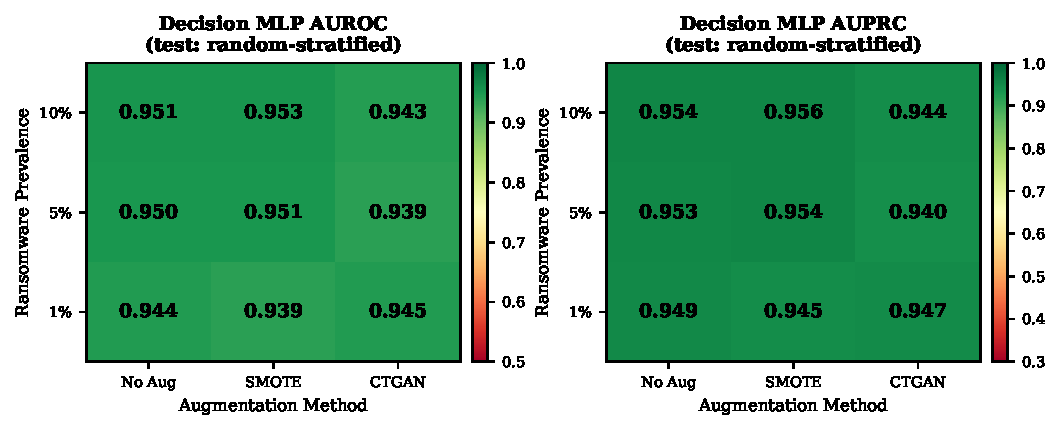
\includegraphics[width=\columnwidth]{Figures/fig_ef_ctgan_ablation.pdf}
  \caption{Decision MLP AUROC (left) and AUPRC (right) under induced class
    imbalance at $10\%$, $5\%$, and $1\%$ ransomware prevalence across three
    augmentation conditions. AUROC is robust across all conditions; CTGAN
    provides the strongest calibration recovery at $10\%$ and $5\%$
    prevalence.}
  \label{fig:ef_ctgan_ablation}
\end{figure}

\begin{figure}[h]
  \centering
  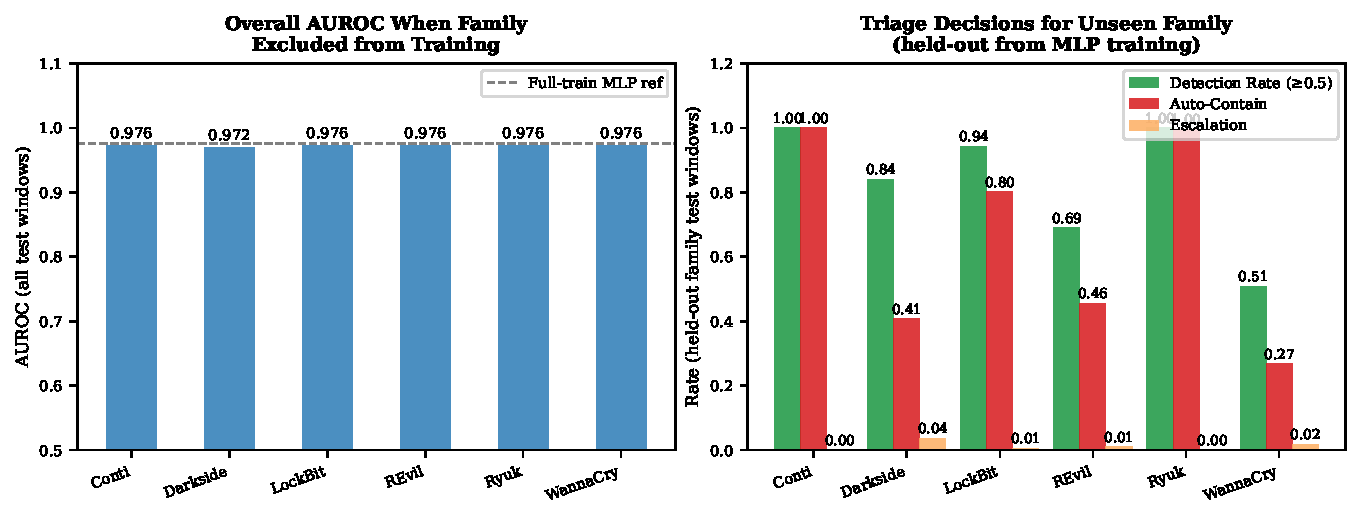
\includegraphics[width=\columnwidth]{Figures/fig_eg_lofo.pdf}
  \caption{Leave-one-family-out evaluation. \emph{Left}: Overall AUROC (all
    test windows) when each ransomware family is excluded from MLP
    training---stable at ${\approx}0.976$ across all holdouts (dashed
    reference). \emph{Right}: Per-family detection rate, auto-contain rate,
    and escalation rate for the held-out family's test windows. Conti and
    Ryuk transfer perfectly; WannaCry and REvil require direct training
    examples for reliable detection.}
  \label{fig:eg_lofo}
\end{figure}

\bibliographystyle{IEEEtran}
\bibliography{Reference_Main}

\end{document}
